\chapter{Usability}
\label{chp:usability}

This chapter will give a brief definition of what usability is, and how user tests can help us improve it. Since the applications are targeted at both children and adults, we will give a description of how the usability tests for these groups will differ.

\section{What is usability?}
\label{sec:usability}
There are many ways to describe the term usability. 

The International Organization for Standardization(ISO) uses the following definition of the term usability\cite{isousability}:

\textit{``Extent to which a system, product or service can be used by specified
users to achieve specified goals with effectiveness, efficiency
and satisfaction in a specified context of use.''}

The same document defines the term ``context of use'' as:

\textit{``Users, tasks, equipment (hardware, software and materials), and
the physical and social environments in which a product is used.''}

These definitions cover how the system is used, the user's thoughts about the use and the context of the system. This can be broken down further into several subgoals in order to achieve better usability, and to give a better insight as to what usability is. 
These subgoals are:

\begin{enumerate}
\item{How precisely is the user able to perform a task by using the application?}
\item{How much resources(for example time, or number of tries) was used to perform the given task using the application?}
\item{How many errors occurred?}
\item{Did the user find the use satisfactory?}
\end{enumerate}

User-centered design is a way of taking extra precautionary measures by having the end user in mind throughout the process. By using this technique the aforementioned goals are achievable. User-centered design is about getting feedback from the users during the design and development process. Being able to imagine how the end user would solve this problem, and consolidate the users when in doubt is a fundamental part of user-centered design. The user's opinion is the measure of how well the system performs and the user's feedback defines how the design scores on usability.


Schneiderman stated eight golden rules in order to achieve a good usability of computer systems\cite{shneiderman2003designing}. In his rules he mentions consistency, informative feedback, reducing short term memory load and permitting easy reversal of actions. These eight golden rules have since their publication become a central part of usability engineering.

Today usability is extremely important in order to achieve success for a system. The users expect a functional and easy-to-use system. From the user's point of view, working with a product which is easily understood, leads to increased productivity, which again may lead to increased sales/usage\cite{folmer2004architecting}. Proper usability engineering may also lead to lower costs for the developers and higher chances for projects being finished on time\cite{nielsen1994usability}. 


\section{How to test usability}
\label{sec:howtotestusability}
There are many approaches to creating a good user experience. Having knowledge of expert opinions is always a good idea, and using user-centered design techniques is also a choice. According to Rubin's handbook of usability testing\cite{rubin2008handbook}, developers should get feedback from users by users tests at different stages of development. According to Rubin, having a user-centered approach will help the developers to address the weakest parts of their system, and give feedback on design decisions. 

A user-centered design can be done in many different ways and at different stages of the product life cycle\cite{abrasusercentereddesign}, as shown in Table \ref{table:designduringlifecycle}:

\begin{table}[H]
\begin{tabular}{|p{5cm} | p{5cm} | p{5cm} |}
\hline
\textbf{Method} & \textbf{Purpose} & \textbf{Phase of the project lifecycle} \\ \hline
Background interviews and questionnaires & To collect data and to understand the user better & When starting the project \\ \hline
Focus groups & Discover design issues and receive feedback & At an early stage \\ \hline
On-site observation & To both collect information of the context the system will be used in, and find the primary problems the users may have & At an early stage \\ \hline
Role playing / simulations & Will give a broader understanding of what the user expects from the system & Early to mid stage of the project \\ \hline
Automated evaluation & Gives feedback on deviations from standards or best practices. This method excludes actual users, but is based on well tested principles & Mid to end of the project \\ \hline
Usability testing & To measure the usability of the system and provide feedback on very specific elements that are poorly designed & Abras\cite{abrasusercentereddesign} says it should be at the end of the project while others\cite{schneidermanusercentered} think it should be done in iterations throughout the project \\ \hline
Interviews and questionnaires & Gives a qualitative measurement of how good or bad the system is & End of the project \\ \hline
\end{tabular}
\caption{Methods of user-centered feedback}
\label{table:designduringlifecycle}
\end{table}


\paragraph{Usability Testing}
The purpose of usability testing is to increase the usability of a system. At the same time, performing these usability tests may save the developers some time and reduce the cost of the project by removing errors and poor design at an early stage\cite{dumas1995practical}.

The usability testing can be performed in different ways\cite{schneidermanusercentered}. At the early stages of the project, low-fidelity prototypes are a good option since they will provide feedback and take proportionally little time to make, making it easier to have more iterations of testing. The different testing methods include a potential user of the system performing tasks to provide real data. Observing and recording each usability test may help the developers to analyze their system, and correct the flaws\cite{dumas1995practical}. 

Before starting the usability tests, the developers should plan goals for what they want to know about the system\cite{isosoftwareengineering}. This will ensure that the purpose of the test is fulfilled. The developers should then plan tasks according to the desired results. These tasks should allow the user to explore the system, or the parts the developers wish to test, giving the test person some time per task, in order not to stress the test person. 

After being planned, the test should be run on a number of different test persons. From Figure \ref{fig:numberoftests}
, you can see that as the number of participants increases, the number of undetected errors decrease. 



 \begin{figure}
 		\centering
 			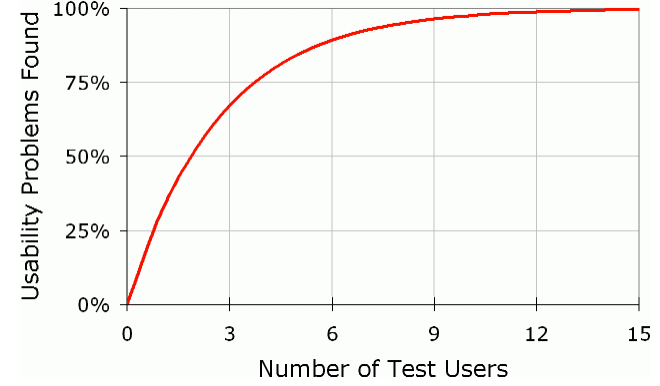
\includegraphics[scale=0.4]{Pictures/app-screenshots/numberoftests.png}
 		\caption{Number of users needed to find percentage of errors according to J. Nielsen\cite{nielsennumberoftests}}
 		 		\label{fig:numberoftests}
 \end{figure}


Nielsen states that after five user tests, 85\% of the errors have been found\cite{nielsennumberoftests}. Molich\cite{molich2008usable} states that six test persons is the ultimate number. Faulkner\cite{faulkner2003beyond} states that while six test persons \textit{may} find 85 \% of the errors, they may also find considerably less. In Faulkner's research, a number of five test users found between 55 \% and 100 \% of the errors, while 20 test persons found between 95 \% and 100 \% of the errors. 

In addition to the practical usability tests, we will use techniques such as background interviews, focus groups and on-site observations. The interviews will be performed in order to achieve a set of control data we can use for comparison when performing later usability test and codesign sessions. As mentioned in \ref{sec:codesign}, we plan on arranging focus group sessions at an early and mid stage of the development of our TUI. These sessions will help us develop our TUI and eliminate usability issues at an early stage. We also plan on using the technique of on-site observation by letting children operate our TUI freely, in order to observe interaction between the children and the TUI. 

\paragraph{Testing environment}
\label{par:testingenvironment}
The next thing to consider when performing usability testing is the testing environment. It should resemble the environment in which the system will be used. To make the most of the tests, it is wise to perform videotaping of the tests. This will help when reviewing the results from the test If the tests are being recorded, a consent from the test person or his/her parent will be required.

Before the test persons arrive, a test leader should be chosen, to guide the test persons through the process. The test leader should be in charge of testing and act as an interviewer to help the participant to ``think-aloud''\cite{lewis1982using}. The test leader should answer questions from the participants, but be careful not to give away information that may affect the results of the test.

After the tasks are done, it is necessary to gather loose ends and obtain answers to all the questions that may remain unanswered. A system usability scale(SUS)\cite{sus} may be a good way to grade the usability of the system together with the observations made during the test. The SUS scale will reflect on how satisfying the usability is in the eyes of the users. Bangor et. al.\cite{susform} have made a scale based on the SUS-forms from different system usability tests, in order to make it possible to compare the mean score of a system with what is an acceptable level of usability. In our testing, we will make use of a Norwegian version, developed by Svan\ae s (see Appendix \ref{app:norsksus}), which will be answered by the test users or the parent of the test user.


\section{How to test usability on children and toddlers}
\label{sec:usabilitytestchildren}
While usability testing on children and toddlers have the same basic approach as testing on adults, there are many more precautions to be followed. 
Hanna et. al.\cite{testingenvironmentforchildren} lays out some of these precautions. They recommend not using children that are skilled with computers since they may find the tasks too easy and will not produce useful data. 
Since children these days have a higher skill with computers thanks to the invasion of tablets and smart phones\cite{babiesusageoftablets}, this may not be great of a concern. 

Since our application is targeted at children with asthma, we want to test the system on children suffering from asthma in addition to children from the same age group, not suffering from asthma. These children will most likely have a different approach to the system and may give different feedback.

Hanna et. al. also point out changes that should be made to the testing environment as mentioned in \ref{par:testingenvironment}. They recommend making the testing environment more suitable for children by placing colourful posters on the walls.
Children of young age may be afraid of ``the Doctor's Office'' and we will need to make adjustments to avoid frightening the children upon their arrival at the test lab. 

As mentioned by Donker and Markopoulos\cite{TalkAloud} talk-aloud is very useful technique when doing usability testing with children. Talk-aloud is a technique were the children talk about what they are doing instead of what they are thinking.

Zaman et. al. proposes a way to measure the likeability of tangible interaction with preschoolers\cite{zaman2007measure}. They based their research on work done by Read, MacFarlane and Casey \cite{read2002endurability}, who found that traditional measures for likeability, for instance a smileyometer, proved to give false results. In fact, Read et. al. found that more than 80\% of the children being tested gave a ``Brilliant'' score. Zaman et. al. implies that children are actually lying when giving these scores, which is understandable from a questionnaire perspective. Instead of using scales as a measure of what is likeable or not, they propose a model where they compare different interaction systems against eachother. They call it the ``This or that'' method. For instance, the interviewer asks the child which system the child prefers, followed by ``this or that'' while pointing to the different systems. We will use a similar approach to understand which forms of interaction children like most.  


\section{Usability testing on mobile devices}
\label{sec:usabilitytestonmobiledevices}
We plan on doing usability testing in testing lab or quiet testing office. The application's main environment for use will be at the user's home, which may be noisier and more hectic than our testing lab. Kaikkonen et. al. states that the similarity between testing environment and place of use is not too important, the test user will still be able to complete the tasks and find the same number of errors cite{kallio2005usability}. This claim is supported by Beck et. al. who discovered that the test persons found more usability problems when sitting down, compared to when walking on the street\cite{beck2003experimental}. 

Schusterich et. al.\cite{schusteritsch2007towards} published a guide on how to build the perfect infrastructure for usability testing on mobile devices, in 2007. They describe how generic infrastructure issues, mobile device-specific issues and usability study context issues should be taken into consideration. Shcusterich et. al. recommends having a number of cameras recording from different angles in order to capture unbiased interaction patterns of the mobile device. 

\subsection{Emulator versus device}
When developing for mobile devices such as Android, it is possible to run an emulator on a pc, instead of running the application on an Android device. The emulator emulates the use of a mobile device on screen. Input must be given by mouse-clicks on buttons/screen elements. The Android emulator emulates use of system resources corresponding to a given Android device, in order to not act faster or slower that a real device. While this may be true in theory, it is not always true in practice. The emulator is often much slower than an actual device.


\begin{figure}
\begin{center}
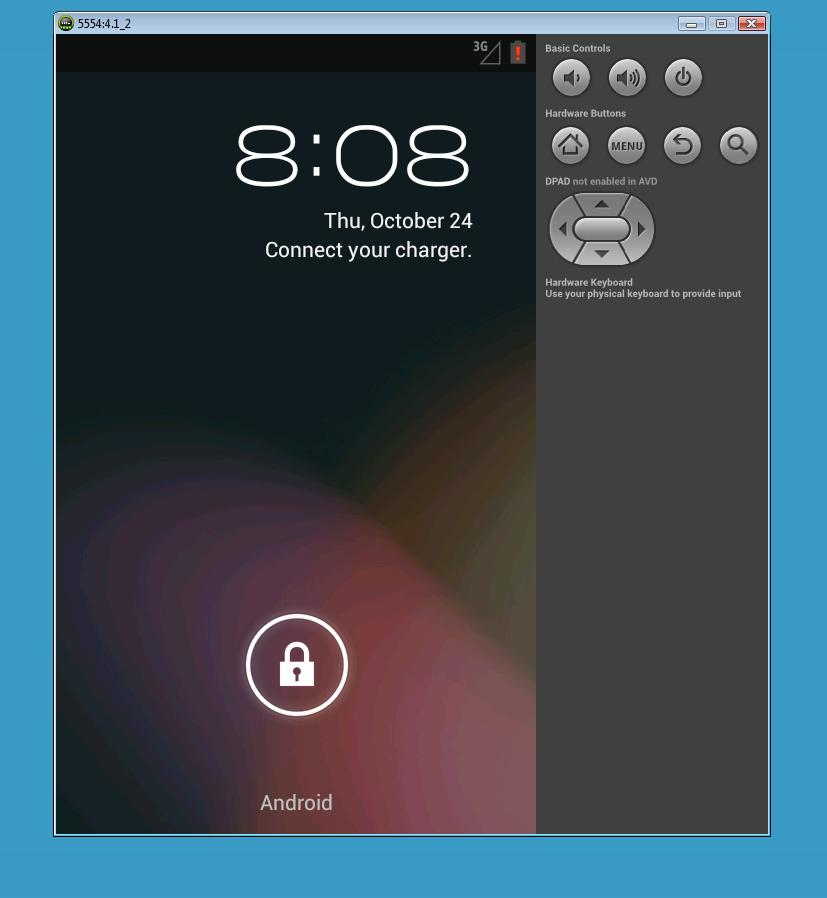
\includegraphics[scale=0.4]{Pictures/app-screenshots/androidemulator.png}
\end{center}
\caption{The Android Emulator running an emulation of Android 4.1}
\label{fig:androidemulator}
\end{figure}

The question arises, should one do usability testing on an emulator or on a real device?
Using the emulator allows for easier capture of the interaction with the device, since it allows screen recording of user input and easier capture of the user when interacting with the emulator. Using a computer as a test object may be more positively perceived by the test user rather than installing the test application on their device or having them doing tests on our device. 

Using a real device has the benefit of being an actual device, and may lead to a more realistic interaction pattern when using the application. While a number of screen recorders for Android devices exist, these require that the device is rooted\fnurl{Android Rooting}{http://en.wikipedia.org/wiki/Android\_rooting} , which is not an option for us. 
The use of a real device also allows the use of gestures, which is a benefit in contrast to the emulator which can simulate swiping. 


Beitol and Cybis\cite{betiol2005usability} compared doing usability testing on a tripod-mounted device to an emulator and using a device in the field. They found that many users found the tripod-mounted device difficult and unnatural to operate. The users found 80\% of the usability issues on the emulator, but Beitol and Cybis points out that use of an emulator may depend on the similarity between the emulator and the device. 



\section{Summary}
\label{sec:usabilitysummary}

The ISO-standards for usability and context of use\cite{isousability} are well known and often mentioned, as they are in fact standards. We aim to achieve a usability as high as possible, through user-centered design and usability testing. 

While we aim to follow Shneidermann's eight golden rules\cite{shneiderman2003designing} when designing AsthmAPP, we focus more on the rules of consistency, informative feedback, reducing short-term memory load and designing dialog to yield closure, rather enabling shortcuts for frequent users (see Chapter \ref{sec:usability-affect-design} for an explanation).

Based on the research we read and the fact that NTNU has an excellent usability test lab at NSEP\fnurl{NSEP Usability lab}{http://www.ntnu.no/nsep/brukbarhetslaboratorium} we decided to do usability testing in doors, with smartphone devices. 